%%%%%%%%%%%%%%%%%%%%%%%%%%%%%%%%%%%%%%%%%%%%%%%%%%%%%%%%%%%%%%%
% JOURNAL INSTRUCTIONS
% This section may be divided by subheadings and should contain sufficient detail so that when read in conjunction with cited references, all procedures can be repeated. For experiments reporting results on animal or human subject research, an ethics approval statement should be included in this section (for further information, see the Bioethics section.)
%%%%%%%%%%%%%%%%%%%%%%%%%%%%%%%%%%%%%%%%%%%%%%%%%%%%%%%%%%%%%%%

%%%%%%%%%%%%%%%%%%%%%%%%%%%%%%%%%
% Questions for 2021-03-09
% - How should we structure: Experimental Design => Results => Discussion
%   - We conducted 3 separate experiments. Currently, we discuss each experiment separately across sections. (1) do we want to stick to this structure? (2) if so, what should the headings be?
% - What parts of what is currently experimental design belong in methods vs. results. vs discussion?
%   - I 100% want to provide some intuition about measurements (in the paper), but where? I'd like trainees to be able to read this as easily as possible. 
% - I do actually think the details for the metrics/measurements are important. 
% - Discuss the overall flow of the methods section. Should the 'quantifying tape of life' metrics actually be under experiment 1 since that's what they are relevant to?
% - I think we could combine results and discussion? Other major re-organizations?
% - 'mutation accumulation'
%%%%%%%%%%%%%%%%%%%%%%%%%%%%%%%%%

\section{Materials and Methods}

% -- bookmark --

\subsection{The Avida Digital Evolution Platform}

% We conducted our study using the Avida Digital Evolution Platform \citep{ofria_avida:_2009}. 
% Avida provides a computational study system where populations of digital organisms undergo Darwinian evolution, allowing researchers to test hypotheses that would be difficult or impossible to address in natural systems.

% - Define digital organisms -
Avida is a study system wherein self-replicating computer programs (digital organisms) compete for space on a finite toroidal grid \citep{ofria_avida:_2009}.
Each digital organism is defined by a linear sequence of program instructions (its genome) and a set of virtual hardware components used to interpret and express those instructions. 
% Avida tracks each organism as it expresses its genome in a given environment in order to measure that organism's phenotype.
Genomes are expressed sequentially except when the execution of one instruction deterministically changes which instruction should be executed next (e.g., a `jump' instruction). 
Genomes are built using an instruction set that is both robust (\textit{i.e.}, any ordering of instructions is syntactically valid, though not necessarily meaningful) and Turing Complete (\textit{i.e.}, able to represent any computable function, though not necessarily in an efficient manner) [cite].
% ; that is, any ordering of instructions is syntactically valid (though not necessarily meaningful), and genomes are able to represent any computable function (though not necessarily in an efficient manner).
The instruction set includes operations for basic computations, flow control (e.g., conditional logic and looping), input, output, and self-replication.
% @AML: Outsource the next sentence to a figure!
% The virtual hardware set includes components such as a central processing unit (CPU) for executing instructions, registers to store values, buffers for inputs and outputs, and memory stacks \citep{ofria_avida:_2009}.

% \begin{figure}[h!]
    \centering
    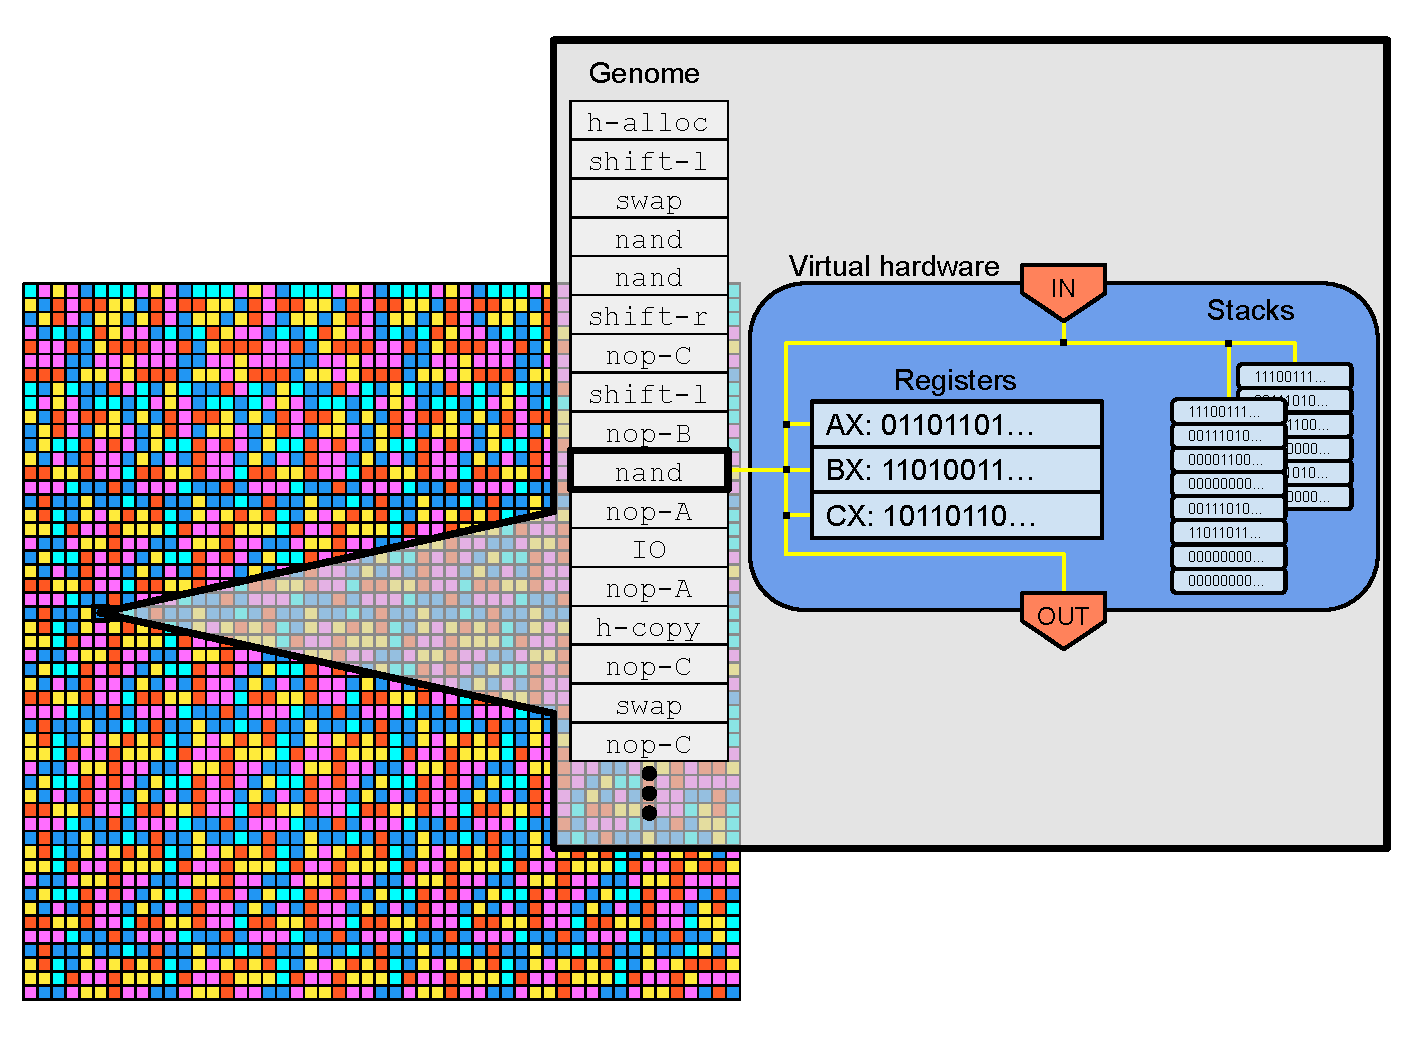
\includegraphics[width=\textwidth]{media/avida-hardware.pdf}
    \caption{\small
    \textbf{todo.}
    todo.
    }
    \label{fig:avida-virtual-hardware}
\end{figure}

% Feedback:
%  - make grid non-repetitive
%    - as tile rotate
%  - output a task? 
%    - one of first 6


% - define reproduction & mutation -
Organisms in Avida reproduce asexually by copying their genome instruction-by-instruction and then dividing. 
However, copy operations are imperfect and can result in single-instruction substitution mutations in an offspring's genome. 
For this work, we configured copy operations to err at a rate of one expected mutation for every 400 instructions copied (i.e, a per-instruction error rate of 0.0025).
% at a per-instruction rate of 0.0025 (i.e., one mutation expected for every 400 instructions copied).
We held individual genomes at a fixed length of 100 instructions; that is, we did not include insertion and deletion mutations. 
We used fixed-length genomes to control for treatment-specific conditions resulting in the evolution of substantially different genome sizes [supplement, citations]\footnote{We repeated our experiments without genome size restrictions and observed qualitatively similar results [cite supplement].}, which could, on its own, drive differences in evolutionary outcomes among experimental treatments.
When an organism divides in Avida, its offspring is placed in a random location on the toroidal grid, replacing any previous occupant.
For this work, we used the default 60 by 60 grid size, which limits the maximum population size to 3600 organisms.
As such, improvements to the speed of self-replication are advantageous in the competition for space.
% The combination of this competition for space and heritable variation from imperfect replication results in evolution by natural selection.

% Avida tracks each organism as it expresses its genome in a given environment in order to measure that organism's phenotype.

% - define fitness/metabolic rate/improving replication speed -
During evolution, organism replication rates improve in two ways: by improving genome efficiency (e.g., using a more compact encoding) or by accelerating the rate at which the genome is expressed (their ``metabolic rate'').
An organism's metabolic rate determines the speed at which it executes instructions in its genome.
Initially, an organism's metabolic rate is proportional to the length of its genome, but that rate is adjusted as it completes designated tasks, such as performing Boolean logic computations \citep{ofria_avida:_2009}.
In this way, we can reward or punish particular phenotypic traits. 

\subsubsection{Phenotypic plasticity in Avida}

%%%% TODO - EDIT THIS SECTION

% -- Phenotypes & Phenotypic plasticity --
% - What is a phenotype in Avida
In this work, we measure a digital organism's phenotype as the set of Boolean logic functions that it performs in a given environment.
Sensory instructions in the Avida instruction set allow organisms to detect how performing a particular logic function would affect their metabolic rate [cite - supplement]. 
We define a phenotypically plastic organism as one that uses sensory information to alter which logic functions it performs based on the environment.

% -- Adaptive plasticity & non-adaptive plasticity --
Phenotypic plasticity in Avida can be adaptive or non-adaptive for a given set of environments.
Adaptive plasticity shifts net task expression closer to the optimum for the given environments.
% Non-adaptive plasticity either changes task expression in a neutral way or further from the optimum for a given set of environments.
Non-adaptive plasticity changes task expression in either a neutral or deleterious way.% for a given set of environments.
Optimal plasticity changes tasks to always perfectly match the set of rewarded tasks.% for each environment.

% For the majority of our experiments, we focus on the following 6 one- and two-input logic functions: NOT, NAND, AND, OR-NOT, OR, and AND-NOT. 
% An organism's \textit{comprehensive} or \textit{aggregate} phenotype is characterized by the set of logic functions performed in each of a set of given environments. 

% \vspace{1cm}
% \subsubsection{Evolving adaptive phenotypic plasticity in Avida}
% \label{sec:methods:evolution-of-plasticity-in-avida}

% @AML: Based on Nkrumah's feedback, I think this section needs to be reorganized. 
\vspace{0.7cm}
\subsection{Experimental design}
\label{sec:methods:experiment}

%%%%%%%%%%%%%%%%%%%%%%%%%%%%%%%%%%%%%%%%%%%%%%%%%
% OUTLINE
%%%%%%%%%%%%%%%%%%%%%%%%%%%%%%%%%%%%%%%%%%%%%%%%%
% Overview of experimental design - with diagram (not a subsubsection?)
% - Focused around diagram
% Environment implementations
% Specifications for Phase 1
% specifications for Phase 2A
% specifications for Phase 2B
% specifications for Phase 2C
% Measurements and Analyses
% - number of coalescence
% - mutation accumulation
% - phenotypic volatility
% - mutational stability
% - genetic architectures
% - novel task performance
% - novel task discovery
%%%%%%%%%%%%%%%%%%%%%%%%%%%%%%%%%%%%%%%%%%%%%%%%%

% -- Overview of experimental design --
We conducted three independent experiments using Avida to investigate how the evolution of adaptive plasticity influences evolutionary outcomes in fluctuating environments.
% @AML: 1 liner of what each of these experiments were? IDK, this info is in the intro, so maybe not important here.
For each experiment, we compared the evolutionary outcomes of populations evolved under three treatments (Figure [XX]): 
(1) a \textbf{PLASTIC} treatment where the environment fluctuates, and digital organisms can use sensory instructions to differentiate between environmental states;
(2) a \textbf{NON-PLASTIC} treatment with identical environment fluctuations, but where sensory instructions are disabled;
and (3) a \textbf{STATIC} control where organisms evolve in a constant environment.

% @AML: maybe cut this next sentence
% These experiments build directly on previous digital evolution studies on the evolution of adaptive phenotypic plasticity \citep{clune_investigating_2007,lalejini_evolutionary_2016} and on the evolutionary consequences of fluctuating environments \citep{wilke_evolution_2001,canino-koning_fluctuating_2019}.
Each experiment was divided into two phases that each lasted for 200,000 updates \footnote{
    One update in Avida is the amount of time required for the average organism to execute 30 instructions. 
    See \citep{ofria_avida:_2009} for more details.
} of evolution (Figure [XX]), which is approximately 30,000 to 40,000 generations.
In phase one of each experiment, we preconditioned populations to their treatment-specific conditions.
% Each experiment shares a common setup for phase one (described in Section \ref{sec:methods:experiment:phase-one}). 
In phase two, we founded new populations with the evolved organisms from phase one and examined their subsequent evolution under given combinations of treatment and experimental conditions.
%In phase two, we examined the subsequent evolution of populations founded with organisms from phase one under given treatment conditions.
% Phase two differed among each of our experiments (described in Sections [X,Y,and Z]). %, depending the goal of the particular experiment.]
During phase two, we tracked each population's evolutionary history as well as saving the full final population.
% , and all comparisons between treatments were performed on these data.
Phase one was for pre-conditioning only; all comparisons between treatments were performed on phase two data. % from populations during phase two.

% -- Phase one => Phase two --
% @AML: I could see these details moving to their respective 'phase sections'!!
% At the beginning of phase one [in each experiment], we founded 100 independent [replicate?] populations for each of three treatment conditions (described below).
% Each phase-one population was founded with a common ancestral strain capable only of self-replication [cite - supplement].
% At the end of phase one, we used the most abundant genotype from each replicate to found a new population for phase two. 
% During phase two, we evolved these new populations in their treatment-specific conditions, tracking their evolutionary history as well as saving the full final population.
% All comparisons between treatments were performed on data from populations during phase two.

\subsubsection{Environments}
\label{sec:methods:experiment:environments}

% ----- ENVIRONMENTS -----
% traits_set_a <- c("not", "and", "or")
% traits_set_b <- c("nand", "ornot", "andnot")

% -- Environment definitions --
We constructed three experimental environments, abbreviated hereafter as ``ENV-A'', ``ENV-B'', and ``ENV-ALL'' ([Figure XX]).
%Six Boolean logic tasks (...) are each rewarded or punished in each environment, as described in Figure YY.
Figure YY describes these environments based on whether each of six Boolean logic tasks (...) is rewarded or punished.
% Each rewarded task performed by an organism doubles their metabolic rate (allowing them to execute twice as many instructions in the same amount of time), and each punished task performed halves their metabolic rate. 
% A task performed by an organism doubles their metabolic rate if it is rewarded (allowing them to execute twice as many instructions in the same amount of time), or halves their metabolic rate if it is punished. 
A rewarded task performed by an organism doubles their metabolic rate, allowing them to execute twice as many instructions in the same amount of time.
A punished task halves an organisms metabolic rate. 


% --- TODO - Move these descriptions to the figure caption ---
% In ENV-A, organisms are rewarded for performing NOT, AND, and OR, but are punished for performing the NAND, OR-NOT, and AND-NOT logic tasks.
% Conversely in ENV-B, organisms are rewarded for performing NAND, OR-NOT, and AND-NOT, but are punished for performing NOT, AND, and OR. 
% Finally, in ENV-ALL, all six tasks are rewarded and none are punished.
% ------------------------------------------------

% @AML: Add deleted text to figure caption.
% Organisms with phenotypes that align with their current environment will quickly outcompete those with mismatched phenotypes.  
% A perfect match in ENV-A or ENV-B will have a metabolic bonus of $\times{8}$, a perfect mismatch will have a penalty of $\times{0.125}$, and an organism that does no tasks or all tasks will not have a modifier at all. 

% -- Treatment-specific environment details --
In both the PLASTIC and NON-PLASTIC conditions, the environment cycles between equal-length periods of ENV-A and ENV-B.
Each of these periods persist for 100 updates (approximately 15 to 20 generations).
Thus, populations experience a total of 1,000 full periods of ENV-A interlaced with 1,000 full periods of ENV-B during each experimental phase.

% -- Sensory instructions + control flow and controlling the capacity for plasticity --
% @AML: Not description of an environment, but it is how organisms sense the environment. Not sure where else this would go.
Organisms in the PLASTIC treatments differentiate between ENV-A and ENV-B by executing one of six sensory instructions, each associated with a particular logical task; these sensory instructions detect whether their associated task is currently rewarded or punished (see Supplemental Section [blah] for details [cite]).
By using sensory information in combination with execution flow-control instructions, organisms can conditionally perform different logic tasks depending on the current environmental conditions.

\subsubsection{Experiment Phase 1 -- Environment preconditioning}
\label{sec:methods:experiment:phase-one}
% @AML: if we use 'phase 1' and 'phase 2X' in headings, should we switch all 'phase one' text to 'phase 1' etc?

For each treatment, we founded 100 independent populations from a common ancestral strain capable only of self-replication [cite - supplement].
% Each phase-one population was founded with a common ancestral strain capable only of self-replication [cite - supplement].
%Phase one gives populations time (200,000 updates) to adapt to their treatment conditions, affording adaptive phenotypic plasticity the opportunity to evolve \textit{de novo} in the PLASTIC treatment.
At the end of phase one, we extracted the most abundant (i.e., dominant) genotype from each replicate population to found a new population for phase two.

%The evolution of adaptive phenotypic plasticity is not a guaranteed outcome in phase one of the PLASTIC treatment.
For the PLASTIC treatment, we measure plasticity by independently testing a given genotype in each of ENV-A and ENV-B.
We discard phase one populations if the dominant genotype does not exhibit optimal plasticity.
% @AML: not sure this is the *best* way to define optimal plasticity (it misses on it being okay if the genome performs neutral tasks).
% An optimally plastic genotype expresses only the NOT, AND, and OR logic functions in ENV-A and performs only the OR-NOT, OR, and AND-NOT in ENV-B.
% An optimally plastic genotype expresses each of the rewarded tasks in a given environment and none of the punished tasks in that environment.
This approach ensures that measurements taken on PLASTIC-treatment populations during the second phase of each experiment reflect the evolutionary consequences of adaptive plasticity.
%are representative of populations with adaptive phenotypic plasticity.

% We consider a genotype to be plastic if it expresses a different set of tasks when [tested/cultured] in ENV-A than when [tested] in ENV-B.
% Genotypes labeled \textit{optimally} plastic express each of the rewarded tasks in a given environment and none of the punished tasks in that environment.

% ---bookmark---

\subsubsection{Experiment Phase 2A -- Evolutionary change rate}
% Testing evolutionary change

% To test whether the evolution of adaptive plasticity
% constrains the rate of subsequent evolutionary change, we 
% [1 sentence of motivation/hypothesis?].
Phase two continued exactly as phase one, except we tracked the rates of evolutionary change in each of the PLASTIC-, NON-PLASTIC-, and STATIC-treatment populations. 
Specifically, we quantified evolutionary change rates using four metrics (defined in Section [X]):
(1) number of coalescence events,
(2) mutation accumulation, 
(3) phenotypic volatility,
and (4) mutational stability.
We additionally examined how the genetic architectures of organisms and their ancestors changed over time.  

\subsubsection{Experiment Phase 2B -- Novel task evolution}

% [1 sentence of motivation/hypothesis?].
Phase two continued exactly as phase one, except we used the expanded task set of 77 Boolean logic tasks during the second phase of evolution \citep{ofria_avida:_2009}.
This task set includes the six phase one tasks (NOT, NAND, AND, OR-NOT, OR, and AND-NOT; hereafter called ``base'' tasks) plus 71 new phase two tasks (hereafter called ``novel'' tasks).
Under all experimental treatments, organisms could improve their metabolic rate by performing any of the 71 novel tasks.
The six base tasks were still present in the environment and continued to be rewarded or punished according to the particular treatment conditions.
% @AML: line below is cut-able if necessary
As such, in fluctuating environments, the six base tasks continued to fluctuate, but the additional 71 tasks were always rewarded; in static environments, performing any of the 77 logic tasks was always beneficial.
% @AML: not sure where this next sentence belongs
During this experiment, we tracked the extent to which populations evolving under each treatment were capable of acquiring and retaining novel tasks.  

An organism received a \novelTraitsReward\ metabolic rate improvement for each of the novel tasks it performed (limited to one reward per unique task).
This reward provided a selective pressure to evolve these tasks, but their benefits did not overwhelm existing treatment-specific selective pressures.
As such, populations in the PLASTIC and NON-PLASTIC treatments could not easily escape environmental fluctuations by abandoning the fluctuating base tasks.

\subsubsection{Experiment Phase 2C -- Deleterious instruction accumulation}

% [In this experiment,] we tested the propensity for deleterious instructions to accumulate in genomes under each of the PLASTIC, NON-PLASTIC, and STATIC treatments.
Phase two continued exactly as phase one, except we added a \code{poison} instruction to the instruction set during phase two.
When executed by an organism, the \code{poison} instruction reduces the organism's metabolic rate (and thus reproductive success), but does not otherwise alter the organism's function.
We imposed a 10\% penalty each time an organism executed the \code{poison} instruction, making the instruct explicitly deleterious (see [supplementary material] for tests with 3\% and 30\% penalties, which produced consistent experimental results).
% @AML: want a sentence about what we tracked?
[We measured/tracked the number of times a \code{poison} instruction is executed by each genotype along the dominant lineage (including the final dominant genotype).]

% - measurements -
% @AML: This could get moved to the results?
% At the beginning of phase two, the \code{poison} instruction is not present in the population as it was not part of the instruction set during the first phase of evolution.
% However, by adding \code{poison} to the instruction set during phase two, it can be introduced via a mutation.
% We measured deleterious mutation accumulation by examining the number of times a \code{poison} instruction is executed by each genotype along the dominant lineage (including the final dominant genotype).
% Because the \code{poison} instruction is explicitly deleterious, selection should purge mutations that increase \code{poison} execution in the offspring phenotype.
% As such, we expected such mutations to show up in successful lineages either as accumulated cryptic variation in plastic genomes or via hitchhiking with linked beneficial mutations [cite].

\subsubsection{Measurements and experimental analyses}

% Evolutionary history

% Lineages and phylogenies
% - number of coalescence
% - mutation accumulation
% - phenotypic volatility
% - mutational stability
% - novel task performance
% - novel task discovery
% - genetic architectures

% - How we extracted representative lineages -
For each of our experiments, we tracked and analyzed the phylogenetic histories of evolving populations during phase two. 
For each replicate, we isolated a representative lineage from its founding organism to a member of the dominant (i.e., most abundant) genotype at the end of its evolution.
Because our experimental treatments do not support long-term coexistence, each of these lineages represented the majority of evolutionary history from a given population at the end of our experiment.

% - Measuring evolutionary change -
We quantified rates of evolutionary change using the following four metrics:
(1) number of \textbf{coalescence events} that have occurred, which indicates the frequency of selective sweeps in the population;
(2) \textbf{mutation accumulation}, which is the sum of all mutations that have occurred along a lineage;
(3) \textbf{phenotypic volatility}, which is the number of instances where parent and offspring phenotypes do not match along a lineage, as measured under a given condition;
and (4) \textbf{mutational stability}, which is the proportion of \textit{mutated} offspring along a lineage whose phenotypes do not match that of their parent, as measured under a given condition.

% - Methods for computing volatility -
To calculate phenotypic volatility for a given lineage, we expressed (i.e., evaluated) each genotype along that lineage in a treatment-specific condition, and we summed the number of changes in task profiles between consecutive genotypes.
For lineages evolved in environments fluctuating between ENV-A and ENV-B, we evaluate genotypes in both environmental conditions and count only changes in its \textit{aggregate} phenotype; this technique ensures that environmentally-induced changes are excluded from our measurement.
Phenotypic volatility as defined here illuminates the rate at which accumulated genetic changes actually change the phenotype along a lineage.

% - Methods for computing mutational stability
We measured mutational stability as the fraction of mutated offspring along a given lineage with a different phenotype than their parent.
For lineages evolved in fluctuating environments, we evaluated mutants under both ENV-A and ENV-B and counted all changes in the \textit{aggregate} task profile; like our measure of phenotypic volatility, this technique ensures that environmentally-induced changes are excluded from our measurement.
Mutational stability examines the frequency at which mutations effect changes in an offspring's phenotype.
 
In experiments that introduce novel tasks during phase two, we measured task discovery, task performance, and task loss along representative lineages.
\textbf{Task discovery} measures a given lineage's level of \textit{exploration} of the fitness landscape (i.e., the mapping between genetic space and phenotype space) \citep{canino-koning_fluctuating_2019}. 
We calculated task discovery as the total number of unique tasks ever performed along the lineage, even if a task is later lost; as such, a lineage's task discovery measurement ranged from 0 to 71.

\textbf{Task performance} measures the level of \textit{exploitation} of the fitness landscape at a given point in time.
In this work, we summarized task performance using a count of unique tasks completed by a representative organism from each population.
We focused on an organism from the dominant genotype at the end of the experiment as the most representative phenotype in the evolved population.

\textbf{Task loss} measures how often a lineage fails to retain evolved traits over time and thus indicates the ability for traits to be maintained over time.
We calculated task loss as the number of times along a lineage that a task is performed by a parent but not its offspring. 

% \subsubsubsection{Genetic architectures}

% While Avida clearly defines the mechanics of each instruction, the emergent function of an instruction depends on its context within a genome. 

% @AML: this is a little jarring
For an individual organism, we can perform \textbf{knockout experiments} to identify which instructions are responsible for producing a given phenotypic outcome.
To perform a knockout, we duplicate the organism, replacing a single instruction with an inert ``no-operation'' instruction.
We then identify any phenotypic changes by contrasting the execution results of the ``knockout'' organism and the original.
Such changes provide evidence of the role that the original instruction must have played in the genome.
For example, when an organism performs the NAND task but loses it when an instruction is knocked out, we categorize that instruction as part of the NAND task machinery.
% @AML: maybe move next sentence to results?
We use knockout experiments to characterize the role of each instruction in the genomes of every organism along all study lineages, revealing how genetic architectures change over time.

\vspace{0.5cm}
\subsection{Statistical analyses and software availability}

Across all of our experiments, we differentiated between sample distributions using non-parametric statistical tests.
For each major analysis, we first performed a Kruskal-Wallis test \citep{kruskal_use_1952} to 
determine if there were significant differences in results from the PLASTIC, NON-PLASTIC, and STATIC treatments.
If so, we applied a Wilcoxon rank-sum test \citep{kotz_individual_1992} to distinguish between pairs of treatments.
We applied Bonferroni corrections for multiple comparisons \citep{rice_analyzing_1989} where appropriate.

We conducted our experiments using a modified version of the Avida software, which is open source and freely available on GitHub [cite].
We used Python [cite] for data processing, and we conducted all statistical analyses using R version [x] [cite].
We used the tidyverse collection of R packages [cite] to wrangle data, and we used the following R packages for graphing and visualization: [list and citations].
We used R markdown [cite] and bookdown [cite] to generate web-enabled supplemental material.
All of the source code for our experiments and analyses, including guides for replication and configuration files, can be found in our supplemental material [cite].
Additionally, our experimental data is available on the Open Science framework at [url] [cite].